% =====================================================================
% BMED365: Evaluation of ML Models (E01-E10)
% Beamer presentation in widescreen (16:9)
% =====================================================================
\documentclass[aspectratio=169, 10pt]{beamer}

% =====================================================================
% PACKAGES
% =====================================================================
\usepackage[utf8]{inputenc}
\usepackage[T1]{fontenc}
\usepackage[english]{babel}
\usepackage{graphicx}
\usepackage{tikz}
\usepackage{booktabs}
\usepackage{amsmath}
\usepackage{fontawesome5}
\usepackage{hyperref}
\hypersetup{colorlinks=true, linkcolor=blue, urlcolor=blue}

% =====================================================================
% THEME AND COLORS
% =====================================================================
\usetheme{Madrid}
\usecolortheme{beaver}

% Colors for TikZ diagrams
\definecolor{uibblue}{RGB}{0, 61, 115}
\definecolor{uibred}{RGB}{175, 28, 44}

% =====================================================================
% TITLE INFO
% =====================================================================
\title{Evaluation of ML Models}
\subtitle{BMED365: Topic List E01--E10}
\author{BMED365}
\date{Spring 2026}

% =====================================================================
% DOCUMENT
% =====================================================================
\begin{document}

% ---------------------------------------------------------------------
\begin{frame}
    \titlepage
\end{frame}

% ---------------------------------------------------------------------
\begin{frame}{Overview}
    \begin{enumerate}
        \item \textbf{Confusion Matrix}
        \begin{itemize}
            \item E01--E02: TP, TN, FP, FN
        \end{itemize}
        \item \textbf{Fundamental metrics}
        \begin{itemize}
            \item E03: Accuracy
            \item E04: Precision
            \item E05: Recall / Sensitivity
            \item E06: Specificity
        \end{itemize}
        \item \textbf{Advanced metrics}
        \begin{itemize}
            \item E07: F1-score
            \item E08: ROC curve and AUC
            \item E09: Imbalanced datasets
            \item E10: TRIPOD guidelines
        \end{itemize}
    \end{enumerate}
\end{frame}

% =====================================================================
\section{Confusion Matrix}
% =====================================================================

% ---------------------------------------------------------------------
% E01
% ---------------------------------------------------------------------
\begin{frame}{E01: Interpret a confusion matrix}

    \begin{columns}
        \begin{column}{0.45\textwidth}
            \begin{block}{What is it?}
                Table: predicted vs. actual classes
            \end{block}

            \vspace{2mm}

            \begin{center}
                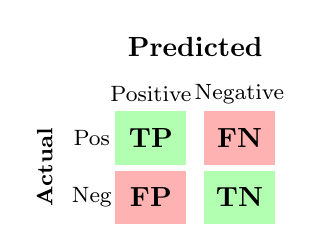
\begin{tikzpicture}[scale=0.75]
                    % Headers
                    \node at (2.25, 3.3) {\textbf{Predicted}};
                    \node at (1.5, 2.5) {\footnotesize Positive};
                    \node at (3, 2.5) {\footnotesize Negative};
                    \node[rotate=90] at (-0.3, 1.25) {\footnotesize\textbf{Actual}};
                    \node at (0.5, 1.75) {\footnotesize Pos};
                    \node at (0.5, 0.75) {\footnotesize Neg};

                    % Boxes
                    \fill[green!30] (0.9,1.3) rectangle (2.1,2.2);
                    \fill[red!30] (2.4,1.3) rectangle (3.6,2.2);
                    \fill[red!30] (0.9,0.3) rectangle (2.1,1.2);
                    \fill[green!30] (2.4,0.3) rectangle (3.6,1.2);

                    \node at (1.5, 1.75) {\textbf{TP}};
                    \node at (3, 1.75) {\textbf{FN}};
                    \node at (1.5, 0.75) {\textbf{FP}};
                    \node at (3, 0.75) {\textbf{TN}};
                \end{tikzpicture}
            \end{center}
        \end{column}
        
        \begin{column}{0.5\textwidth}
            \textbf{Reading the matrix:}
            \begin{itemize}
                \item \textcolor{green!50!black}{\textbf{TP}}: Correct positive
                \item \textcolor{green!50!black}{\textbf{TN}}: Correct negative
                \item \textcolor{red}{\textbf{FP}}: False alarm
                \item \textcolor{red}{\textbf{FN}}: Missed case
            \end{itemize}
            
            \vspace{3mm}
            
            \textbf{Example:} Cancer screening
            \begin{itemize}
                \item TP = Cancer correctly detected
                \item FN = Missed cancer (\textit{dangerous!})
            \end{itemize}
        \end{column}
    \end{columns}
    
\end{frame}

% ---------------------------------------------------------------------
% E02
% ---------------------------------------------------------------------
\begin{frame}{E02: TP, TN, FP, FN in a medical context}
    
    \begin{table}
        \centering
        \begin{tabular}{@{}lp{5cm}p{5cm}@{}}
            \toprule
            \textbf{Term} & \textbf{Definition} & \textbf{Medical example} \\
            \midrule
            \textbf{TP} & Sick patient, model says sick & Cancer correctly identified \\
            \textbf{TN} & Healthy patient, model says healthy & Healthy person confirmed healthy \\
            \textbf{FP} & Healthy patient, model says sick & Unnecessary biopsy \\
            \textbf{FN} & Sick patient, model says healthy & \textcolor{uibred}{Missed cancer} \\
            \bottomrule
        \end{tabular}
    \end{table}
    
    \vspace{5mm}
    
    \begin{alertblock}{Critical question in medicine}
        What is worse: \textbf{False Positive} (FP) or \textbf{False Negative} (FN)?
        \begin{itemize}
            \item Screening: FN is more dangerous (missed disease)
            \item Invasive treatment: FP can be more dangerous (unnecessary risk)
        \end{itemize}
    \end{alertblock}
    
\end{frame}

% =====================================================================
\section{Fundamental Metrics (Accuracy, Precision, Recall, Specificity)}
% =====================================================================

% ---------------------------------------------------------------------
% E03
% ---------------------------------------------------------------------
\begin{frame}{E03: Accuracy}

    \begin{block}{Definition}
        \[
        \text{Accuracy} = \frac{TP + TN}{TP + TN + FP + FN} = \frac{\text{Correct predictions}}{\text{All predictions}}
        \]
    \end{block}

    \vspace{1mm}

    \begin{columns}[T]
        \begin{column}{0.35\textwidth}
            \textbf{Example:}
            \begin{center}
                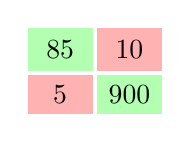
\begin{tikzpicture}[scale=0.55]
                    \fill[green!30] (0,1) rectangle (1.5,2); \node at (0.75, 1.5) {85};
                    \fill[red!30] (1.6,1) rectangle (3.1,2); \node at (2.35, 1.5) {10};
                    \fill[red!30] (0,0) rectangle (1.5,0.9); \node at (0.75, 0.45) {5};
                    \fill[green!30] (1.6,0) rectangle (3.1,0.9); \node at (2.35, 0.45) {900};
                \end{tikzpicture}
            \end{center}
        \end{column}
        \begin{column}{0.6\textwidth}
            \[
            \text{Accuracy} = \frac{85 + 900}{85 + 900 + 10 + 5} = \frac{985}{1000} = 98.5\%
            \]
        \end{column}
    \end{columns}

    \vspace{2mm}

    \begin{alertblock}{Warning}
        High accuracy can be misleading with imbalanced datasets!
    \end{alertblock}

\end{frame}

% ---------------------------------------------------------------------
% E04
% ---------------------------------------------------------------------
\begin{frame}{E04: Precision (PPV)}
    
    \begin{block}{Definition}
        \[
        \text{Precision} = \frac{TP}{TP + FP} = \frac{\text{True positives}}{\text{All predicted positives}}
        \]
    \end{block}
    
    \vspace{3mm}
    
    \textbf{Question:} ``Of all that the model predicts as positive, how many are actually positive?''
    
    \vspace{3mm}
    
    \begin{columns}
        \begin{column}{0.5\textwidth}
            \textbf{High precision is important when:}
            \begin{itemize}
                \item Costly follow-up of positives
                \item Want to avoid false alarms
                \item Example: Rare disease
            \end{itemize}
        \end{column}
        
        \begin{column}{0.45\textwidth}
            \textbf{Example:}
            \[
            \text{Precision} = \frac{85}{85 + 5} = 94.4\%
            \]
            \footnotesize\textit{``94\% of flagged patients are actually sick''}
        \end{column}
    \end{columns}
    
\end{frame}

% ---------------------------------------------------------------------
% E05
% ---------------------------------------------------------------------
\begin{frame}{E05: Recall / Sensitivity}
    
    \begin{block}{Definition}
        \[
        \text{Recall} = \frac{TP}{TP + FN} = \frac{\text{True positives}}{\text{All actual positives}}
        \]
    \end{block}
    
    \vspace{3mm}
    
    \textbf{Question:} ``Of all who are actually positive, how many does the model catch?''
    
    \vspace{3mm}
    
    \begin{columns}
        \begin{column}{0.5\textwidth}
            \textbf{High recall is important when:}
            \begin{itemize}
                \item Severe consequence of missing cases (FN)
                \item Screening for dangerous disease
                \item Example: Cancer screening
            \end{itemize}
        \end{column}
        
        \begin{column}{0.45\textwidth}
            \textbf{Example:}
            \[
            \text{Recall} = \frac{85}{85 + 10} = 89.5\%
            \]
            \textit{``We catch 89.5\% of all cancer cases''}
        \end{column}
    \end{columns}
    
    \vspace{2mm}

    \begin{block}{\footnotesize Other names}
        \footnotesize Recall = Sensitivity = True Positive Rate (TPR)
    \end{block}

\end{frame}

% ---------------------------------------------------------------------
% E06
% ---------------------------------------------------------------------
\begin{frame}{E06: Specificity}
    
    \begin{block}{Definition}
        \[
        \text{Specificity} = \frac{TN}{TN + FP} = \frac{\text{True negatives}}{\text{All actual negatives}}
        \]
    \end{block}
    
    \vspace{3mm}
    
    \textbf{Question:} ``Of all who are actually negative, how many does the model correctly identify?''
    
    \vspace{3mm}
    
    \begin{columns}
        \begin{column}{0.5\textwidth}
            \textbf{High specificity is important when:}
            \begin{itemize}
                \item Want to avoid unnecessary interventions
                \item Costly/risky treatment
                \item Example: Confirmatory tests
            \end{itemize}
        \end{column}
        
        \begin{column}{0.45\textwidth}
            \textbf{Example:}
            \[
            \text{Specificity} = \frac{900}{900 + 5} = 99.4\%
            \]
            \textit{``99.4\% of healthy correctly identified as healthy''}
        \end{column}
    \end{columns}
    
    \vspace{2mm}

    \begin{alertblock}{\footnotesize Trade-off}
        \footnotesize High sensitivity $\leftrightarrow$ Low specificity (and vice versa). Adjusting the threshold affects both.
    \end{alertblock}

\end{frame}

% =====================================================================
\section{Advanced Metrics (F1-score, ROC/AUC, TRIPOD)}
% =====================================================================

% ---------------------------------------------------------------------
% E07
% ---------------------------------------------------------------------
\begin{frame}{E07: F1-score}
    
    \begin{block}{Definition}
        \[
        F1 = 2 \cdot \frac{\text{Precision} \cdot \text{Recall}}{\text{Precision} + \text{Recall}}
        \]
        \textit{Harmonic mean of precision and recall}
    \end{block}
    
    \vspace{3mm}
    
    \textbf{Why harmonic mean?}
    \begin{itemize}
        \item Penalizes extreme values more harshly than arithmetic mean
        \item Precision = 100\%, Recall = 0\% $\rightarrow$ F1 = 0\% (not 50\%!)
    \end{itemize}
    
    \vspace{3mm}
    
    \begin{columns}
        \begin{column}{0.48\textwidth}
            \textbf{When to use F1?}
            \begin{itemize}
                \item Imbalanced datasets
                \item When both FP and FN are important
                \item Comparing models
            \end{itemize}
        \end{column}
        
        \begin{column}{0.48\textwidth}
            \textbf{Example:}
            \[
            F1 = 2 \cdot \frac{0.944 \cdot 0.895}{0.944 + 0.895} = 0.92
            \]
        \end{column}
    \end{columns}
    
\end{frame}

% ---------------------------------------------------------------------
% E08
% ---------------------------------------------------------------------
\begin{frame}{E08: ROC curve and AUC}
    
    \begin{columns}
        \begin{column}{0.45\textwidth}
            \textbf{ROC curve:}
            \begin{itemize}
                \item \textbf{R}eceiver \textbf{O}perating \textbf{C}haracteristic
                \item Plots TPR vs. FPR for different thresholds
                \item Shows trade-off between sensitivity and specificity
            \end{itemize}
            
            \vspace{3mm}
            
            \textbf{AUC (Area Under Curve):}
            \begin{itemize}
                \item Area under the ROC curve
                \item Value between 0 and 1
                \item AUC = 0.5: random guessing
                \item AUC = 1.0: perfect classification
            \end{itemize}
        \end{column}
        
        \begin{column}{0.5\textwidth}
            \begin{center}
                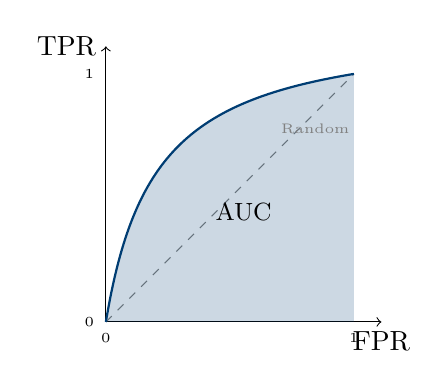
\begin{tikzpicture}[scale=0.7]
                    \draw[->] (0,0) -- (5,0) node[below] {FPR};
                    \draw[->] (0,0) -- (0,5) node[left] {TPR};
                    
                    % Diagonal (random)
                    \draw[dashed, gray] (0,0) -- (4.5,4.5);
                    
                    % Good ROC curve
                    \draw[uibblue, thick] (0,0) .. controls (0.5,3) and (1.5,4) .. (4.5,4.5);
                    
                    % Fill area
                    \fill[uibblue, opacity=0.2] (0,0) .. controls (0.5,3) and (1.5,4) .. (4.5,4.5) -- (4.5,0) -- cycle;
                    
                    \node at (2.5, 2) {\small AUC};
                    \node[gray] at (3.8, 3.5) {\tiny Random};
                    
                    % Axis labels
                    \node at (0, -0.3) {\tiny 0};
                    \node at (4.5, -0.3) {\tiny 1};
                    \node at (-0.3, 0) {\tiny 0};
                    \node at (-0.3, 4.5) {\tiny 1};
                \end{tikzpicture}
            \end{center}
        \end{column}
    \end{columns}
    
    \vspace{3mm}
    
    \begin{block}{Rule of thumb}
        AUC $>$ 0.9: Excellent \quad AUC 0.8--0.9: Good \quad AUC 0.7--0.8: Fair \quad AUC $<$ 0.7: Poor
    \end{block}
    
\end{frame}

% ---------------------------------------------------------------------
% E09
% ---------------------------------------------------------------------
\begin{frame}{E09: When accuracy is insufficient}
    
    \textbf{The problem with imbalanced datasets:}
    
    \vspace{3mm}
    
    \begin{columns}
        \begin{column}{0.5\textwidth}
            \textbf{Example:} 1000 patients
            \begin{itemize}
                \item 950 healthy, 50 sick
                \item Model predicts ALL as healthy
            \end{itemize}
            
            \vspace{3mm}
            
            \textbf{Results:}
            \[
            \text{Accuracy} = \frac{950}{1000} = 95\%
            \]
            \[
            \text{Recall} = \frac{0}{50} = 0\%
            \]
            
            \textbf{High accuracy, but useless model!}
        \end{column}
        
        \begin{column}{0.45\textwidth}
            \textbf{Solutions:}
            \begin{itemize}
                \item Use F1-score or AUC
                \item Focus on recall for screening
                \item Report all metrics
                \item Compare with baseline
            \end{itemize}
            
            \vspace{3mm}
            
            \textbf{Techniques for imbalance:}
            \begin{itemize}
                \item Oversampling (SMOTE)
                \item Undersampling
                \item Class weights
                \item Stratified splitting
            \end{itemize}
        \end{column}
    \end{columns}
    
\end{frame}

% ---------------------------------------------------------------------
% E10
% ---------------------------------------------------------------------
\begin{frame}{E10: \href{https://www.tripod-statement.org/}{TRIPOD} Guidelines}

    \begin{block}{What is TRIPOD?}
        \textbf{T}ransparent \textbf{R}eporting of a multivariable prediction model for \textbf{I}ndividual \textbf{P}rognosis \textbf{O}r \textbf{D}iagnosis
    \end{block}
    
    \vspace{3mm}
    
    \textbf{Key points for reporting ML in medicine:}
    
    \begin{columns}
        \begin{column}{0.48\textwidth}
            \begin{enumerate}
                \item Clear description of study population
                \item Define outcomes and predictors clearly
                \item Describe missing data handling
                \item Report model development in detail
            \end{enumerate}
        \end{column}
        
        \begin{column}{0.48\textwidth}
            \begin{enumerate}
                \setcounter{enumi}{4}
                \item Internal validation (cross-validation)
                \item External validation if possible
                \item Report calibration and discrimination
                \item Discuss limitations
            \end{enumerate}
        \end{column}
    \end{columns}
    
    \vspace{5mm}
    
    \begin{alertblock}{Why is it important?}
        TRIPOD ensures \textbf{reproducibility} and \textbf{quality control} of prediction models in health research.
    \end{alertblock}
    
\end{frame}

% ---------------------------------------------------------------------
% Summary
% ---------------------------------------------------------------------
\begin{frame}{Summary: E01--E10}

    \begin{columns}[T]
        \begin{column}{0.35\textwidth}
            \begin{center}
                \textbf{Confusion Matrix}\\[2mm]
                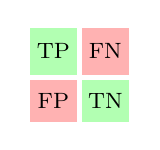
\begin{tikzpicture}[scale=0.6]
                    \fill[green!30] (0,1) rectangle (1,2); \node at (0.5, 1.5) {\footnotesize TP};
                    \fill[red!30] (1.1,1) rectangle (2.1,2); \node at (1.6, 1.5) {\footnotesize FN};
                    \fill[red!30] (0,0) rectangle (1,0.9); \node at (0.5, 0.45) {\footnotesize FP};
                    \fill[green!30] (1.1,0) rectangle (2.1,0.9); \node at (1.6, 0.45) {\footnotesize TN};
                \end{tikzpicture}
            \end{center}
        \end{column}
        \begin{column}{0.30\textwidth}
            \textbf{Metrics:}\\[1mm]
            \footnotesize
            Recall = $\frac{\text{TP}}{\text{TP}+\text{FN}}$\\[2mm]
            Precision = $\frac{\text{TP}}{\text{TP}+\text{FP}}$\\[2mm]
            Specificity = $\frac{\text{TN}}{\text{TN}+\text{FP}}$
        \end{column}
        \begin{column}{0.30\textwidth}
            \textbf{Advanced:}\\[1mm]
            \footnotesize
            \textbf{F1-score:}\\
            Combines Precision + Recall\\[2mm]
            \textbf{ROC/AUC:}\\
            Overall picture independent of threshold
        \end{column}
    \end{columns}

    \vspace{3mm}

    \begin{block}{\footnotesize Key points}
        \footnotesize
        \begin{itemize}
            \item Choose metric based on medical context (FN vs. FP consequences)
            \item Accuracy is often insufficient - use F1, AUC, precision, recall
            \item ROC/AUC gives overall picture independent of threshold
            \item Follow \href{https://www.tripod-statement.org/}{TRIPOD} for transparent reporting
        \end{itemize}
    \end{block}

\end{frame}

\end{document}
